
\documentclass[a4paper]{article}
\usepackage{amsfonts}
\usepackage{amsmath}
\usepackage{amssymb}
\usepackage{graphicx}     
\newcommand{\ddx}{\dfrac{d}{dx}}
\newcommand{\ddg}{\dfrac{d}{dg}}

\begin{document}
  
\noindent \large Auteur: Luca Letroye \\
\noindent \large Studierichting: Informatica\\
\noindent \large Oefeningenreeks 5G nr. 9.\

\medskip

\normalsize

$y^2 = x^4 + x^5 = x^4(1+x)$\\

$x^4(1+x) \geq 0$ als $x \geq -1 $\\

$x^4(1+x) < 0$ als $x < -1 $\\

$V = \pi \displaystyle\int_{-1}^0(x^4+x^5)dx$\\

$ = \pi \left( \displaystyle\int_{-1}^0x^4dx + \displaystyle\int_{-1}^0x^5dx\right)$\\

$ = \pi \left(\left[\dfrac{x^5}{5}\right]_{-1}^0 + \left[\dfrac{x^6}{6}\right]_{-1}^0  \right)$\\

$V = \pi \left(\dfrac{1}{5} - \dfrac{1}{6}\right) = \dfrac{\pi}{30}$


\begin{figure}[h]
\centering
	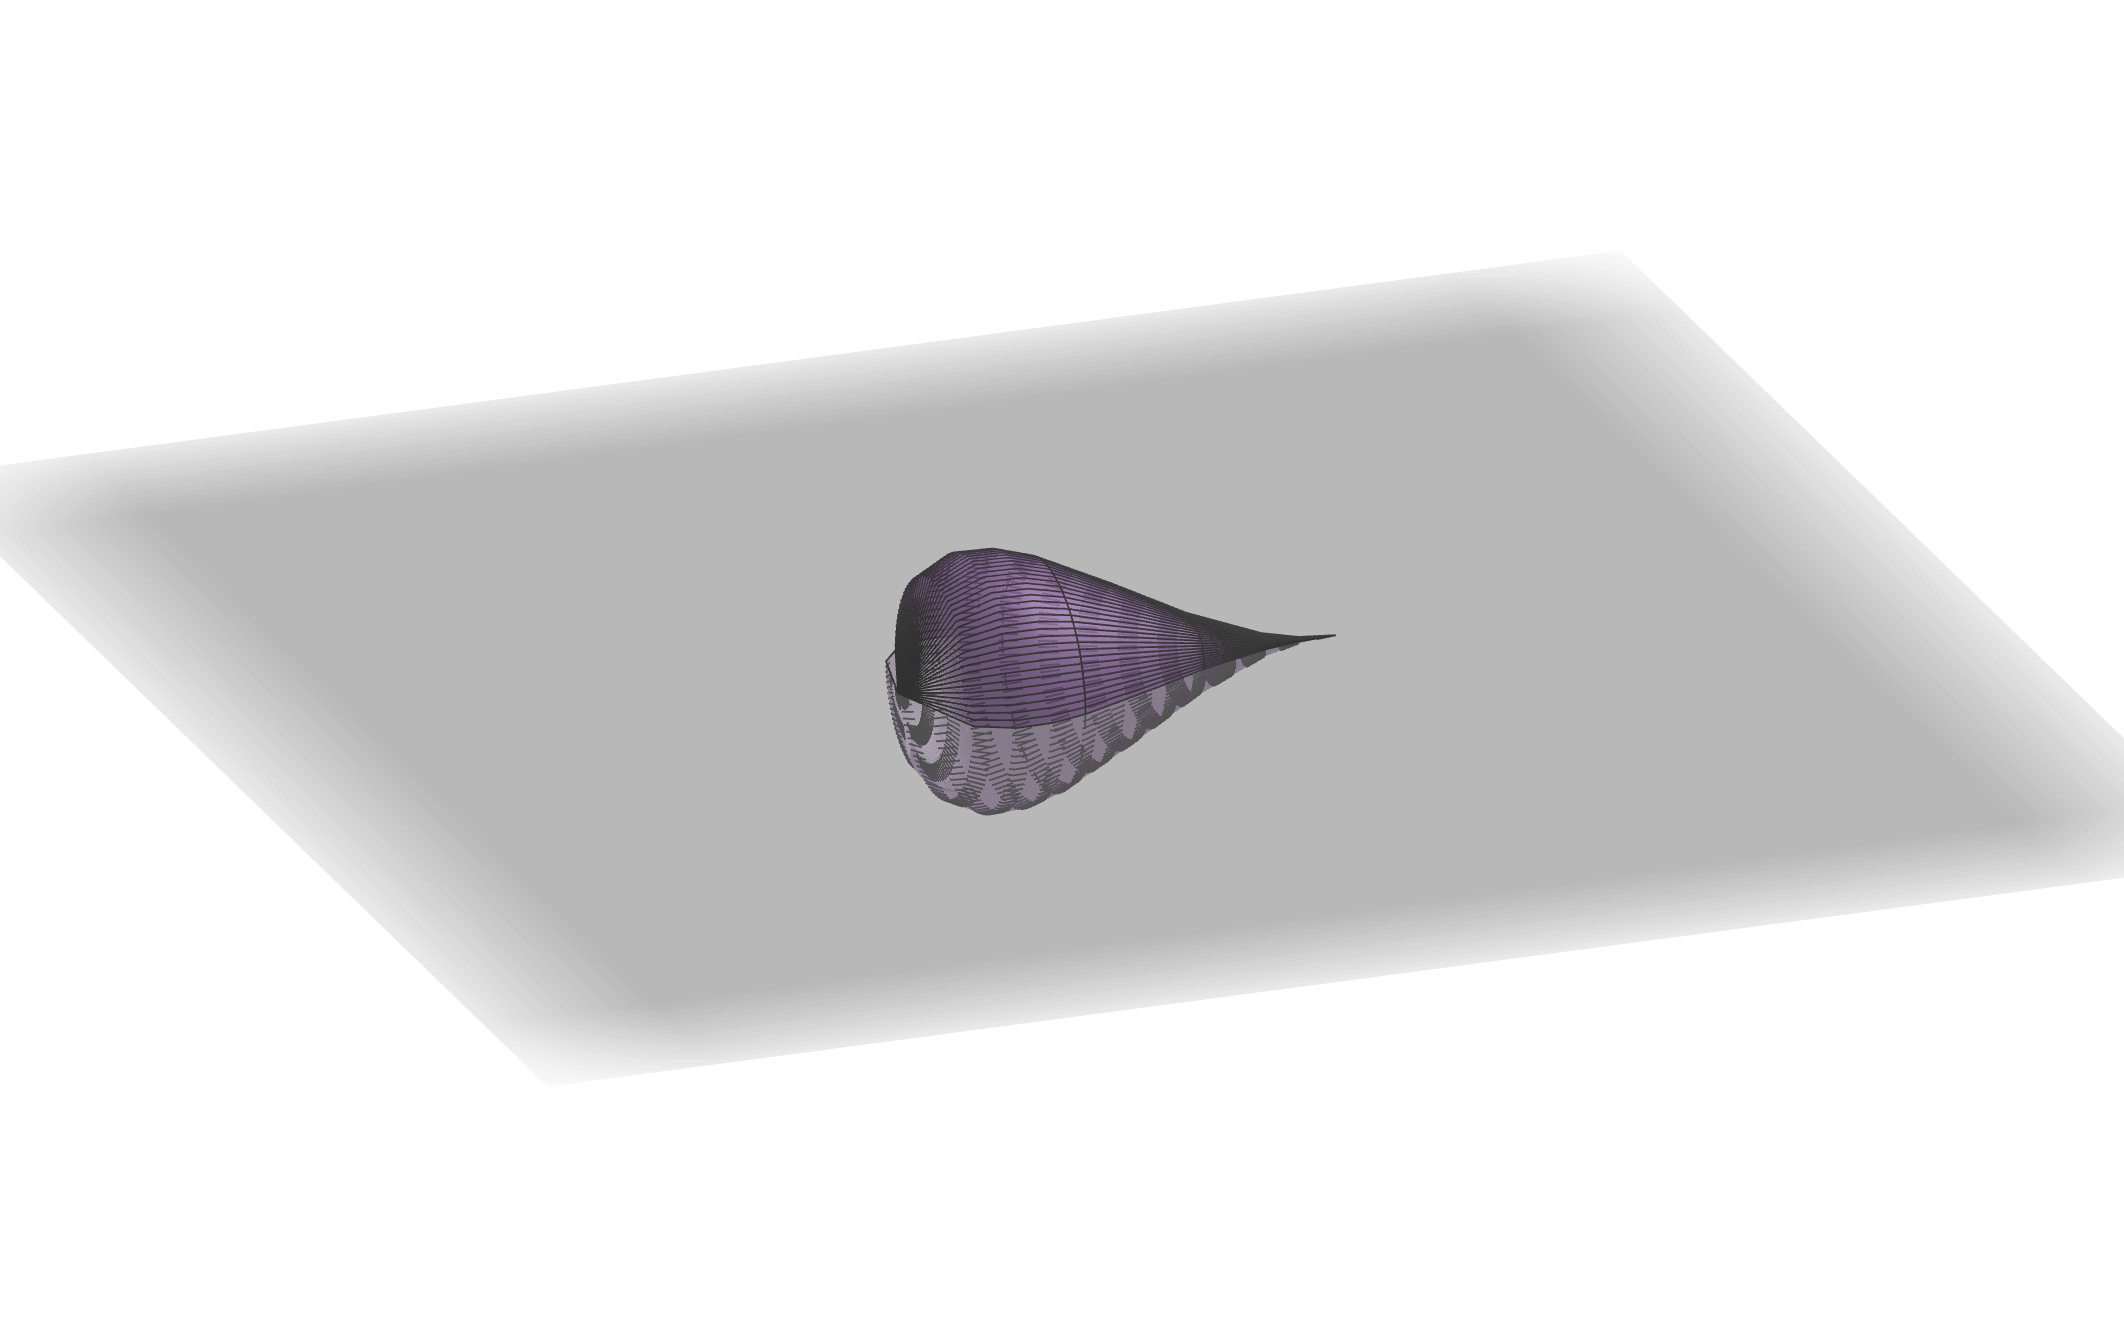
\includegraphics[width=6cm]{5G-9-luca.letroye.INF.png}
\end{figure}




\begin{thebibliography}{999}
%\bibitem{a} Referentie
\end{thebibliography}

\end{document}
